\documentclass[a4paper,12pt, uplatex, dvipdfmx]{jsarticle}
\usepackage{amsmath,amsthm,amssymb,amsfonts,fancyhdr, enumerate, setspace, braket, emathEy, graphicx}

\newcommand{\ds}{\displaystyle}

\theoremstyle{definition}
\newtheorem{theorem}{定理}
\newtheorem*{theorem*}{定理}
\newtheorem*{definition}{定義}
\newtheorem{lemma}{補題}
\newtheorem{example}{例}
\newtheorem*{remark}{注意}
\newtheorem*{promis}{約束}
\renewcommand{\proofname}{証明}
\renewcommand{\thesection}{\arabic{section}}

\renewcommand{\arraystretch}{1.3}



\chead{8.3  練習問題解答 }
\lhead{}
\rhead{}

\pagestyle{fancy}

\begin{document}



\begin{enumerate}[(1)]

  \setlength{\itemsep}{1zh}

\item  $\ds \iint_{D} \sin (x+y) \ dx dy, \quad D=\Set{(x,y) | 0 \leqq y \leqq \frac{\pi}{2}, \; 0 \leqq x \leqq y}$
  \[
    \begin{aligned}
      \iint_{D} \sin (x+y) \ dx dy &= \int_{0}^{\frac{\pi}{2}} \left( \int_{0}^{y} \sin (x+y) \ dx \right) dy
      = \int_{0}^{\frac{\pi}{2}} \Big[ -\cos (x+y)\Big]_{x=0}^{x=y} dy\\
      &= \int_{0}^{\frac{\pi}{2}} \left( -\cos(2y) + \cos y \right) dy=1
    \end{aligned}
  \]
  \begin{figure}[h]
    \centering
    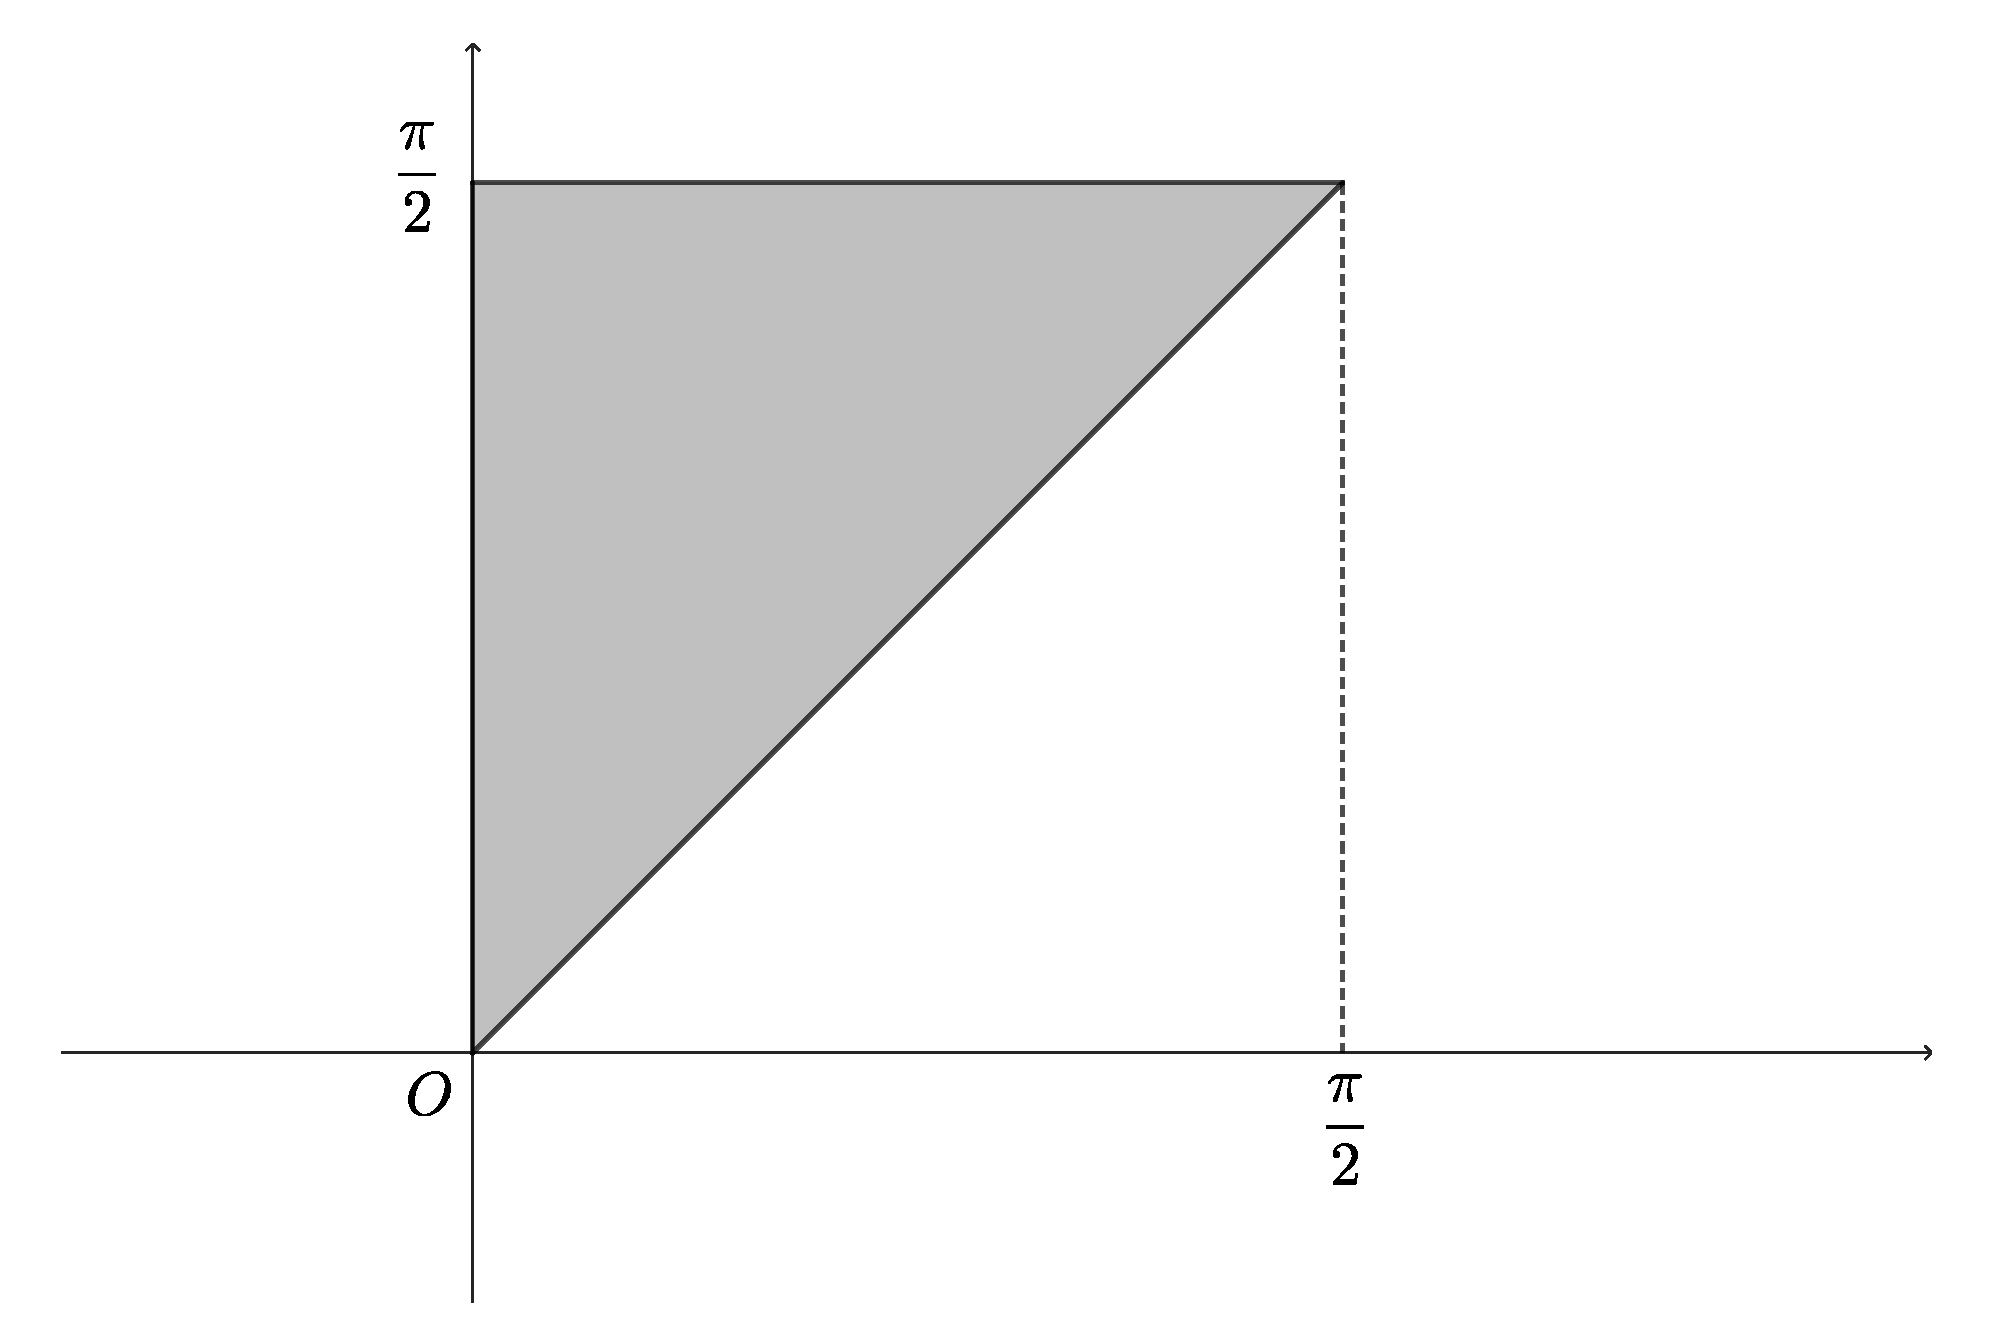
\includegraphics[height=4.5cm]{./pictures/fig1.pdf}
  \end{figure}

\item $\ds \iint_{D} x \ dx dy, \quad D=\Set{(x,y) | y \leqq x \leqq \sqrt{y}}$
  \vspace{1zh}

  $D$ は横線集合として $D=\Set{(x,y) | 0 \leqq x \leqq 1, \; x^2 \leqq y \leqq x}$ と書ける.
  \[
    \begin{aligned}
      \iint_{D}x \ dx dy &= \int_{0}^{1} \left( \int_{x^2}^{x} x \ dy \right) dx
      =\int_{0}^{1} \Big[xy \Big]_{y=x^2}^{y=x} \ dx
      = \int_{0}^{1}\left( x^2-x^3\right) dx = \frac{1}{12}
    \end{aligned}
  \]
  \begin{figure}[h]
    \centering
    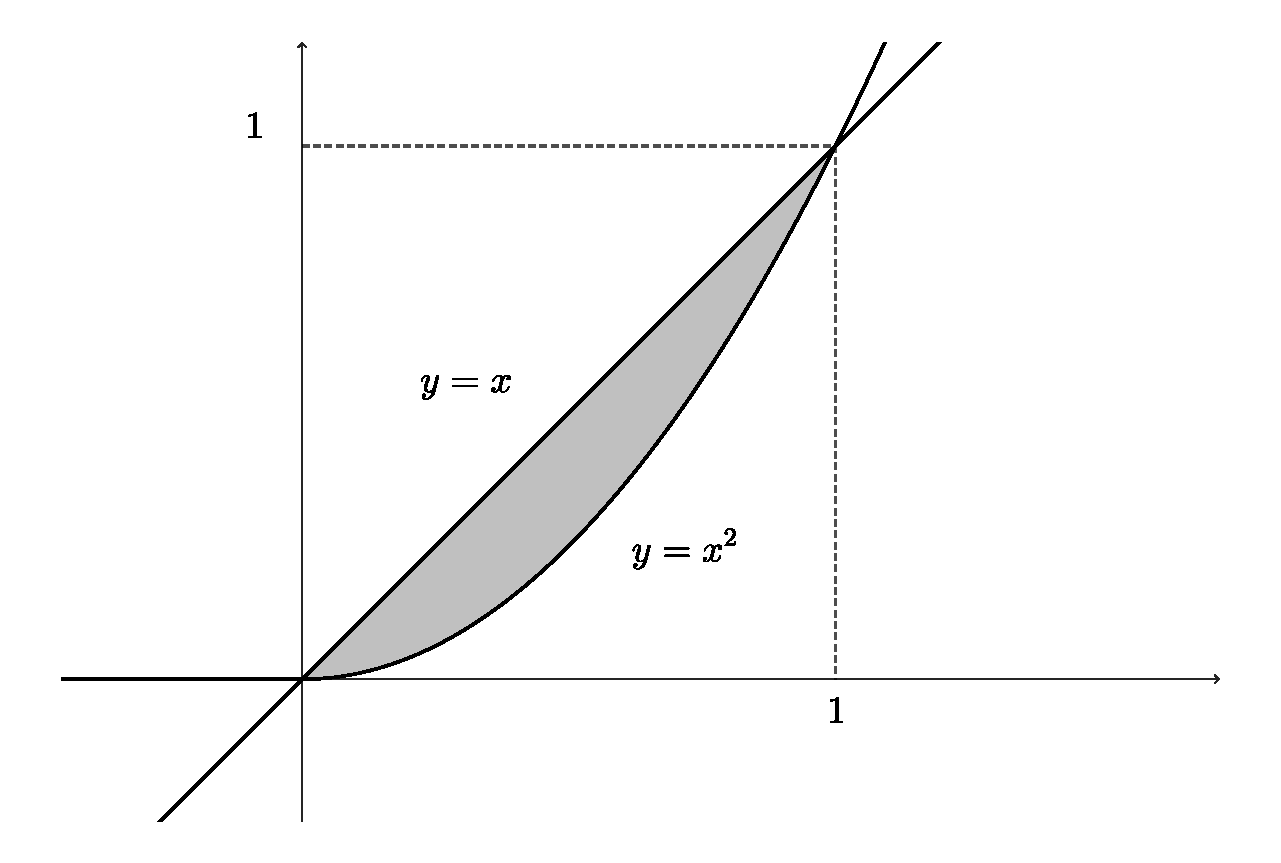
\includegraphics[height=4.5cm]{./pictures/fig2.pdf}
  \end{figure}

 
\item $\ds \iint_{D} xy \ dx dy, \quad D=\Set{(x,y) | x+y \leqq 2, \; y^2 \leqq x, \; 0 \leqq y}$

  \vspace{1zh}

  $D$ は横線集合として $D=\Set{(x,y) | 0 \leqq y \leqq 1, \; y^2 \leqq x \leqq 2-y}$ と書ける.
  \[
    \begin{aligned}
      \iint_{D} x y \ dx dy & \int_{0}^{1}\left( \int_{y^2}^{2-y} xy \ dx \right) dy
      = \int_{0}^{1}\left[\frac{x^2y}{2}\right]_{x=y^2}^{x=2-y} \ dy\\
      &= \frac{1}{2}\int_{0}^{1}\left( -y^5+y^3-4y^2+4y\right) dy = \frac{3}{8}
    \end{aligned}
  \]
    \begin{figure}[h]
    \centering
    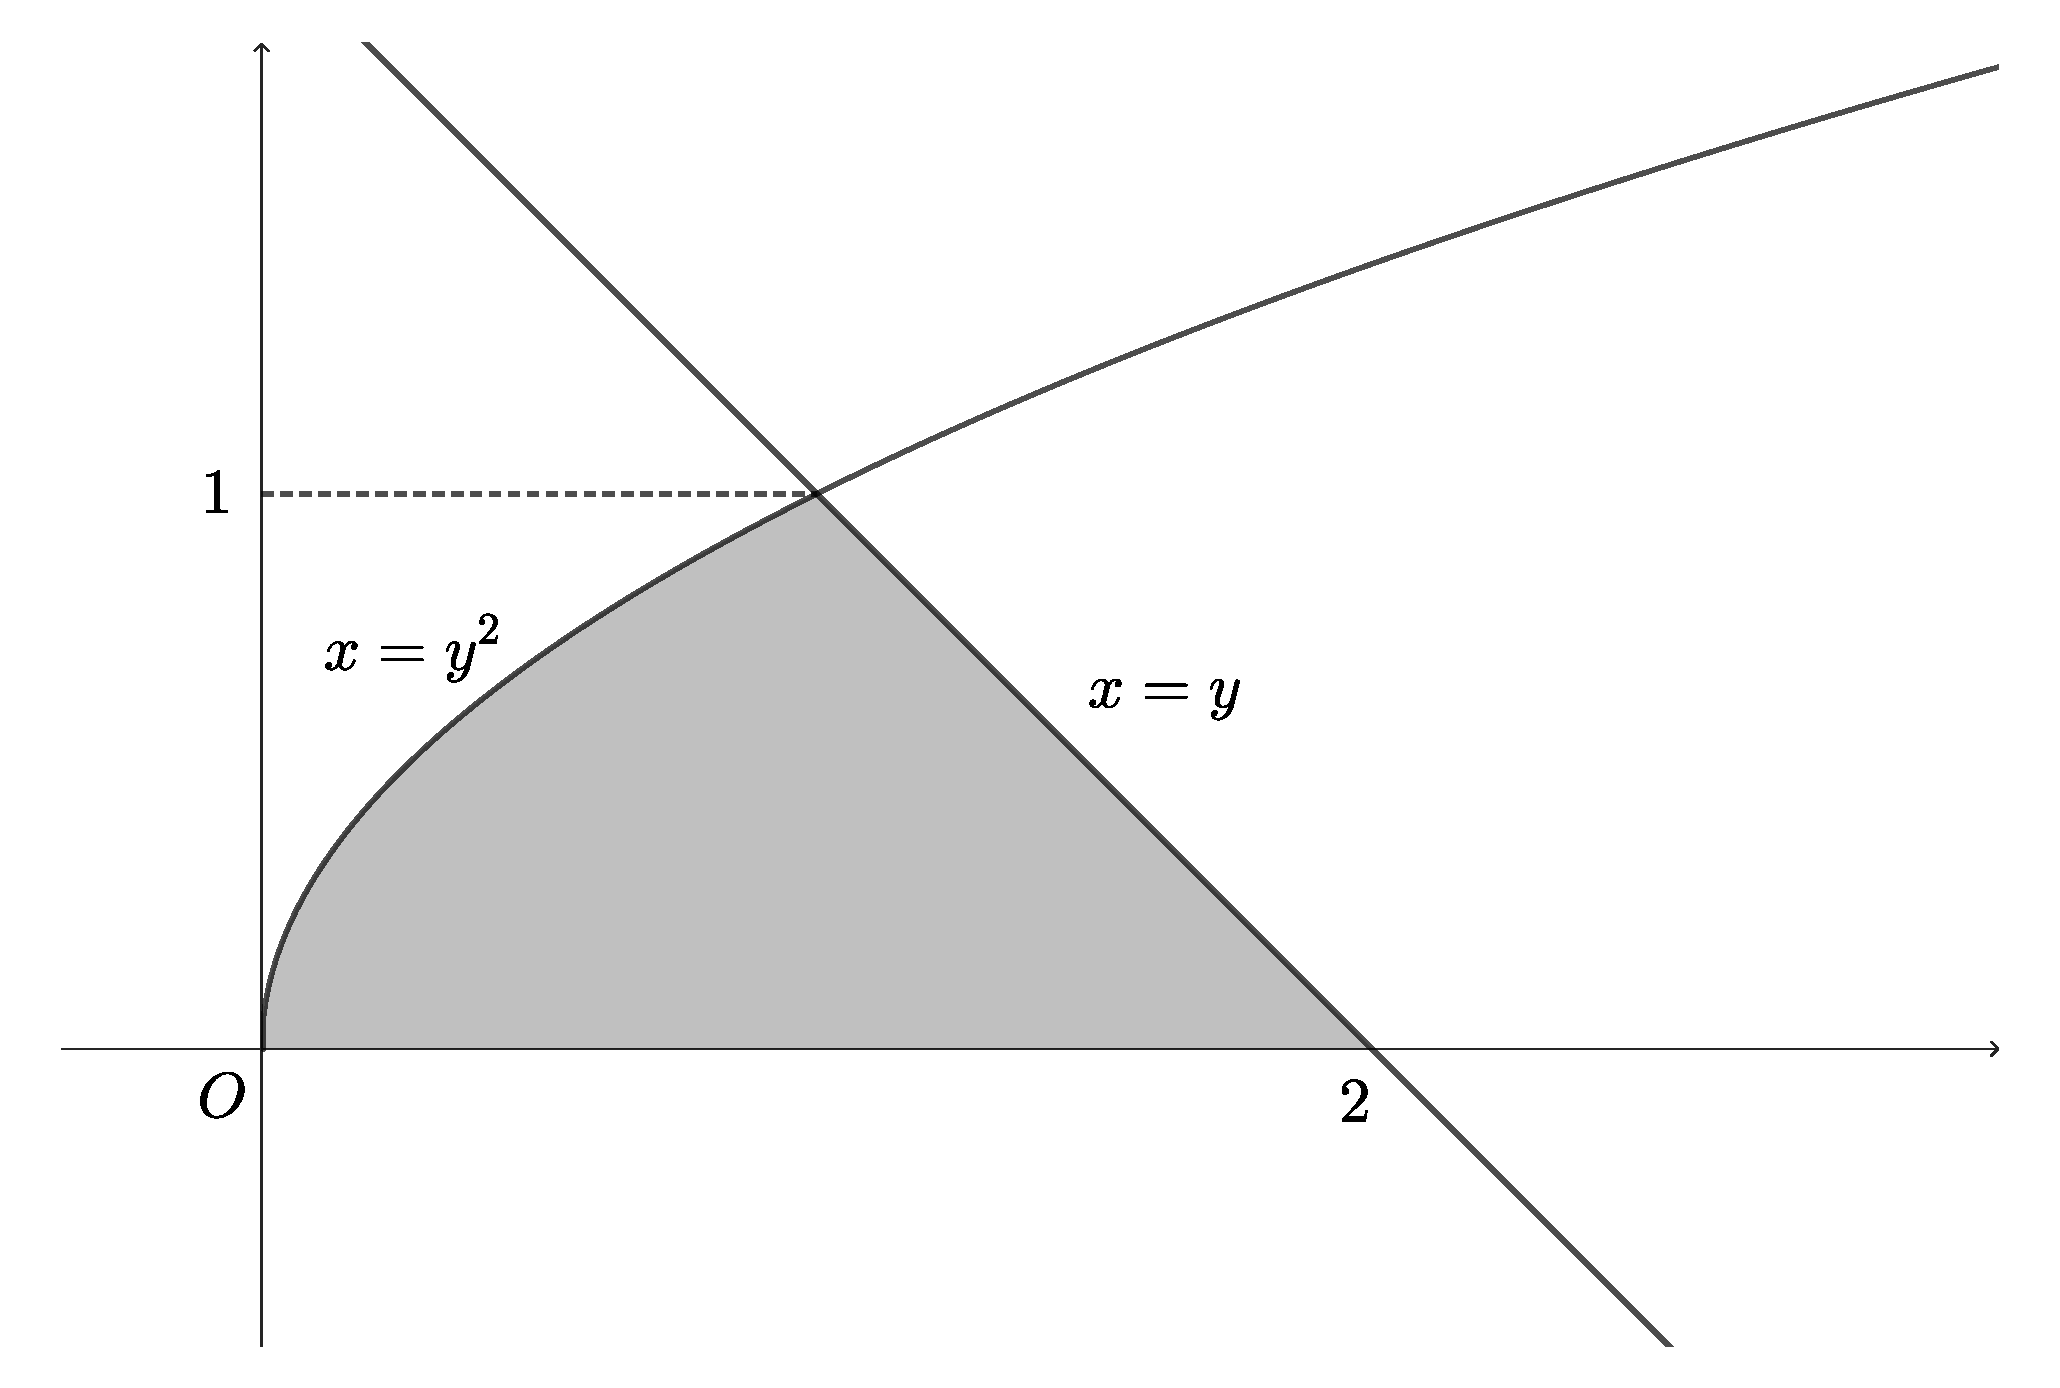
\includegraphics[height=4cm]{./pictures/fig3.pdf}
  \end{figure}


\item $\ds \iint_{D} \sin\left( \pi x^2\right) \ dx dy, \quad D=\Set{(x,y) | y \leqq x \leqq 1, \; 0 \leqq y \leqq 1}$

  \vspace{1zh}

  $D$ は縦線集合として $D=\Set{(x,y) | 0 \leqq x \leqq 1, \; 0 \leqq y \leqq x}$ と書ける.
  \[
    \begin{aligned}
      \iint_{D} \sin\left( \pi x^2\right) \ dx dy &= \int_{0}^{1}\left( \int_{0}^{x} \sin\left( \pi x^2\right) dy \right) dx
      = \int_{0}^{1} \sin\left(\pi x^2\right) \Big[ y \Big]_{y=0}^{y=x} \ dx\\
      &= \int_{0}^{1} x \sin \left( \pi x^2 \right) dx = \frac{1}{\pi}
    \end{aligned}
  \]
  \begin{figure}[h]
    \centering
    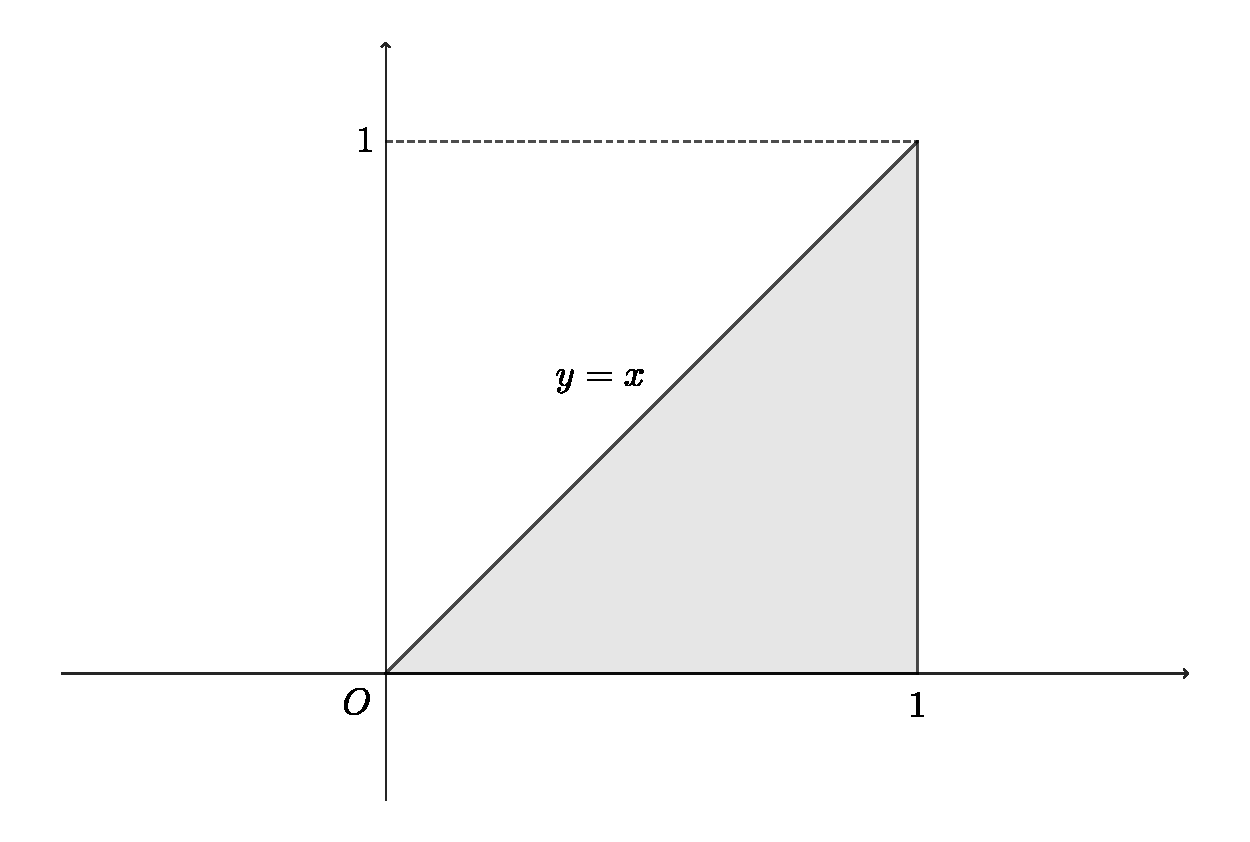
\includegraphics[height=4cm]{./pictures/fig4.pdf}
  \end{figure}

  
\item $\ds \iint_{D} y \ dx dy, \quad D=\Set{(x,y) | \frac{y}{2} \leqq x \leqq 2y, \; x +y \leqq 1}$

  \vspace{1zh}

  $D$ は縦線集合として
  \[
    D=\Set{(x,y) | 0 \leqq x \leqq \frac{2}{3}, \; \frac{x}{2} \leqq y \leqq \varphi(x)}, \quad \varphi(x) =
    \begin{cases}
      2x & \left( 0 \leqq x \leqq \frac{1}{3}\right)\\
      1-x & \left( \frac{1}{3} \leqq x \leqq \frac{2}{3}\right)
    \end{cases}
  \]
  と書ける.
  \[
    \begin{aligned}
      \iint_{D}y \ dx dy &= \int_{0}^{\frac{2}{3}} \left(
        \int_{\frac{x}{2}}^{\varphi(x)} y \ dy \right) dx =
      \int_{0}^{\frac{1}{3}}\left(\int_{\frac{x}{2}}^{2x} y \ dy
      \right) dx
      + \int_{\frac{1}{3}}^{\frac{2}{3}}\left(\int_{\frac{x}{2}}^{1-x} y \ dy \right) dx\\
      &= \int_{0}^{\frac{1}{3}}
      \left[\frac{y^2}{2}\right]_{y=\frac{x}{2}}^{y=2x} dx +
      \int_{\frac{1}{3}}^{\frac{2}{3}}\left[\frac{y^2}{2}\right]_{y=\frac{x}{2}}^{y=1-x}\ dx\\
      &= \int_{0}^{\frac{1}{3}} \frac{15}{8} x^2 \ dx + \int_{\frac{1}{3}}^{\frac{2}{3}}\left( \frac{3}{8}x^2-x+\frac{1}{2}\right)\ dx
      = \frac{5}{216} + \frac{7}{216} = \frac{1}{18}
    \end{aligned}
  \]
    \begin{figure}[h]
    \centering
    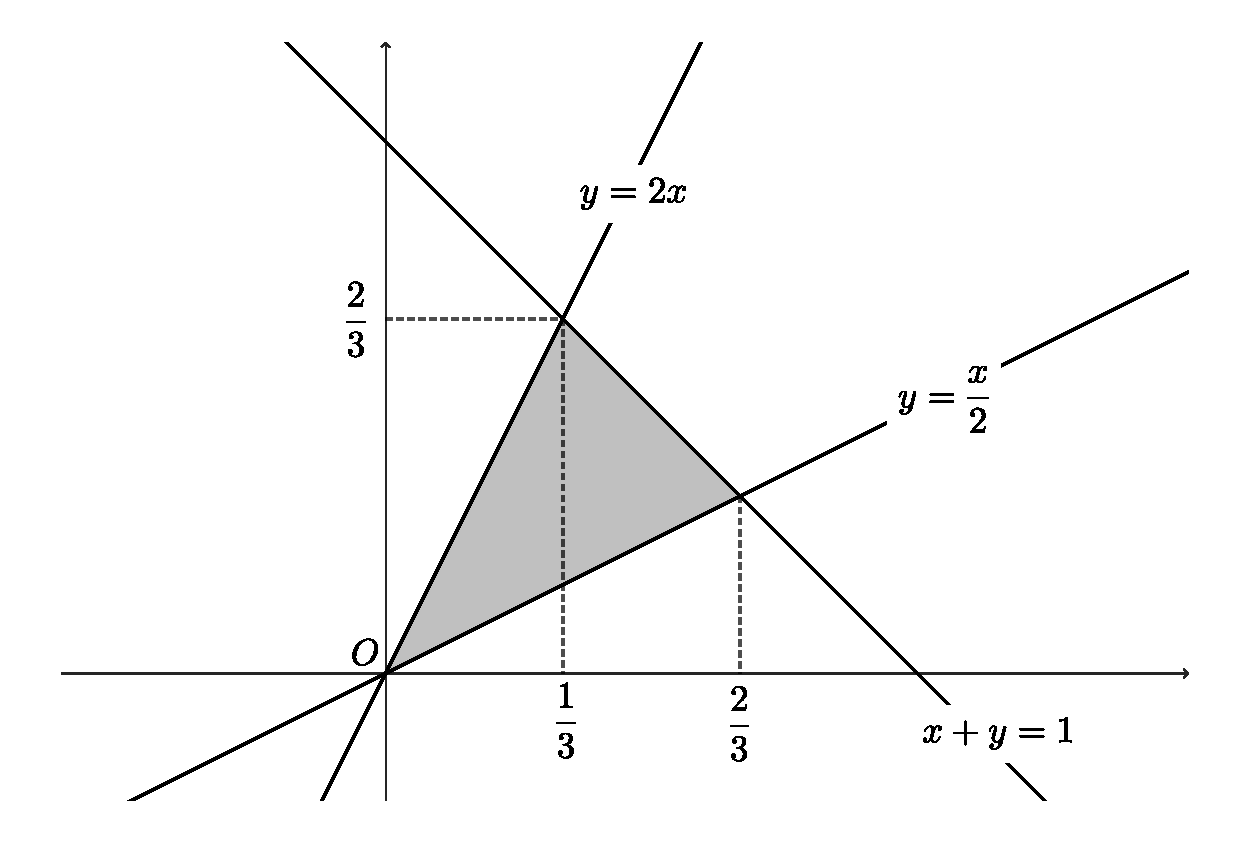
\includegraphics[height=10cm]{./pictures/fig5.pdf}
  \end{figure}

  \newpage
  
\item $\ds \iint_{D} x \ dx dy, \quad D=\Set{(x,y) | -2 \leqq x \leqq 1, \; x^2+4x+1 \leqq y \leqq -x^2+2x+1}$

  \vspace{1zh}

  $D$ は縦線集合として $D=\Set{(x,y) | -1 \leqq x \leqq 0, \; x^2+4x+1 \leqq y \leqq -x^2+2x+1}$ と書ける.
  \[
    \begin{aligned}
      \iint_{D}x \ dx dy &= \int_{-1}^{0}\left( \int_{x^2+4x+1}^{-x^2+2x+1} x \ dy \right) dx
      =\int_{-1}^{0}\Big[ xy \Big]_{y=x^2+4x+1}^{-x^2+2x+1} dx\\
      &= \int_{-1}^{0}\left( -2x^3-2x^2\right) dx = -\frac{1}{6}
    \end{aligned}
  \]
    \begin{figure}[h]
    \centering
    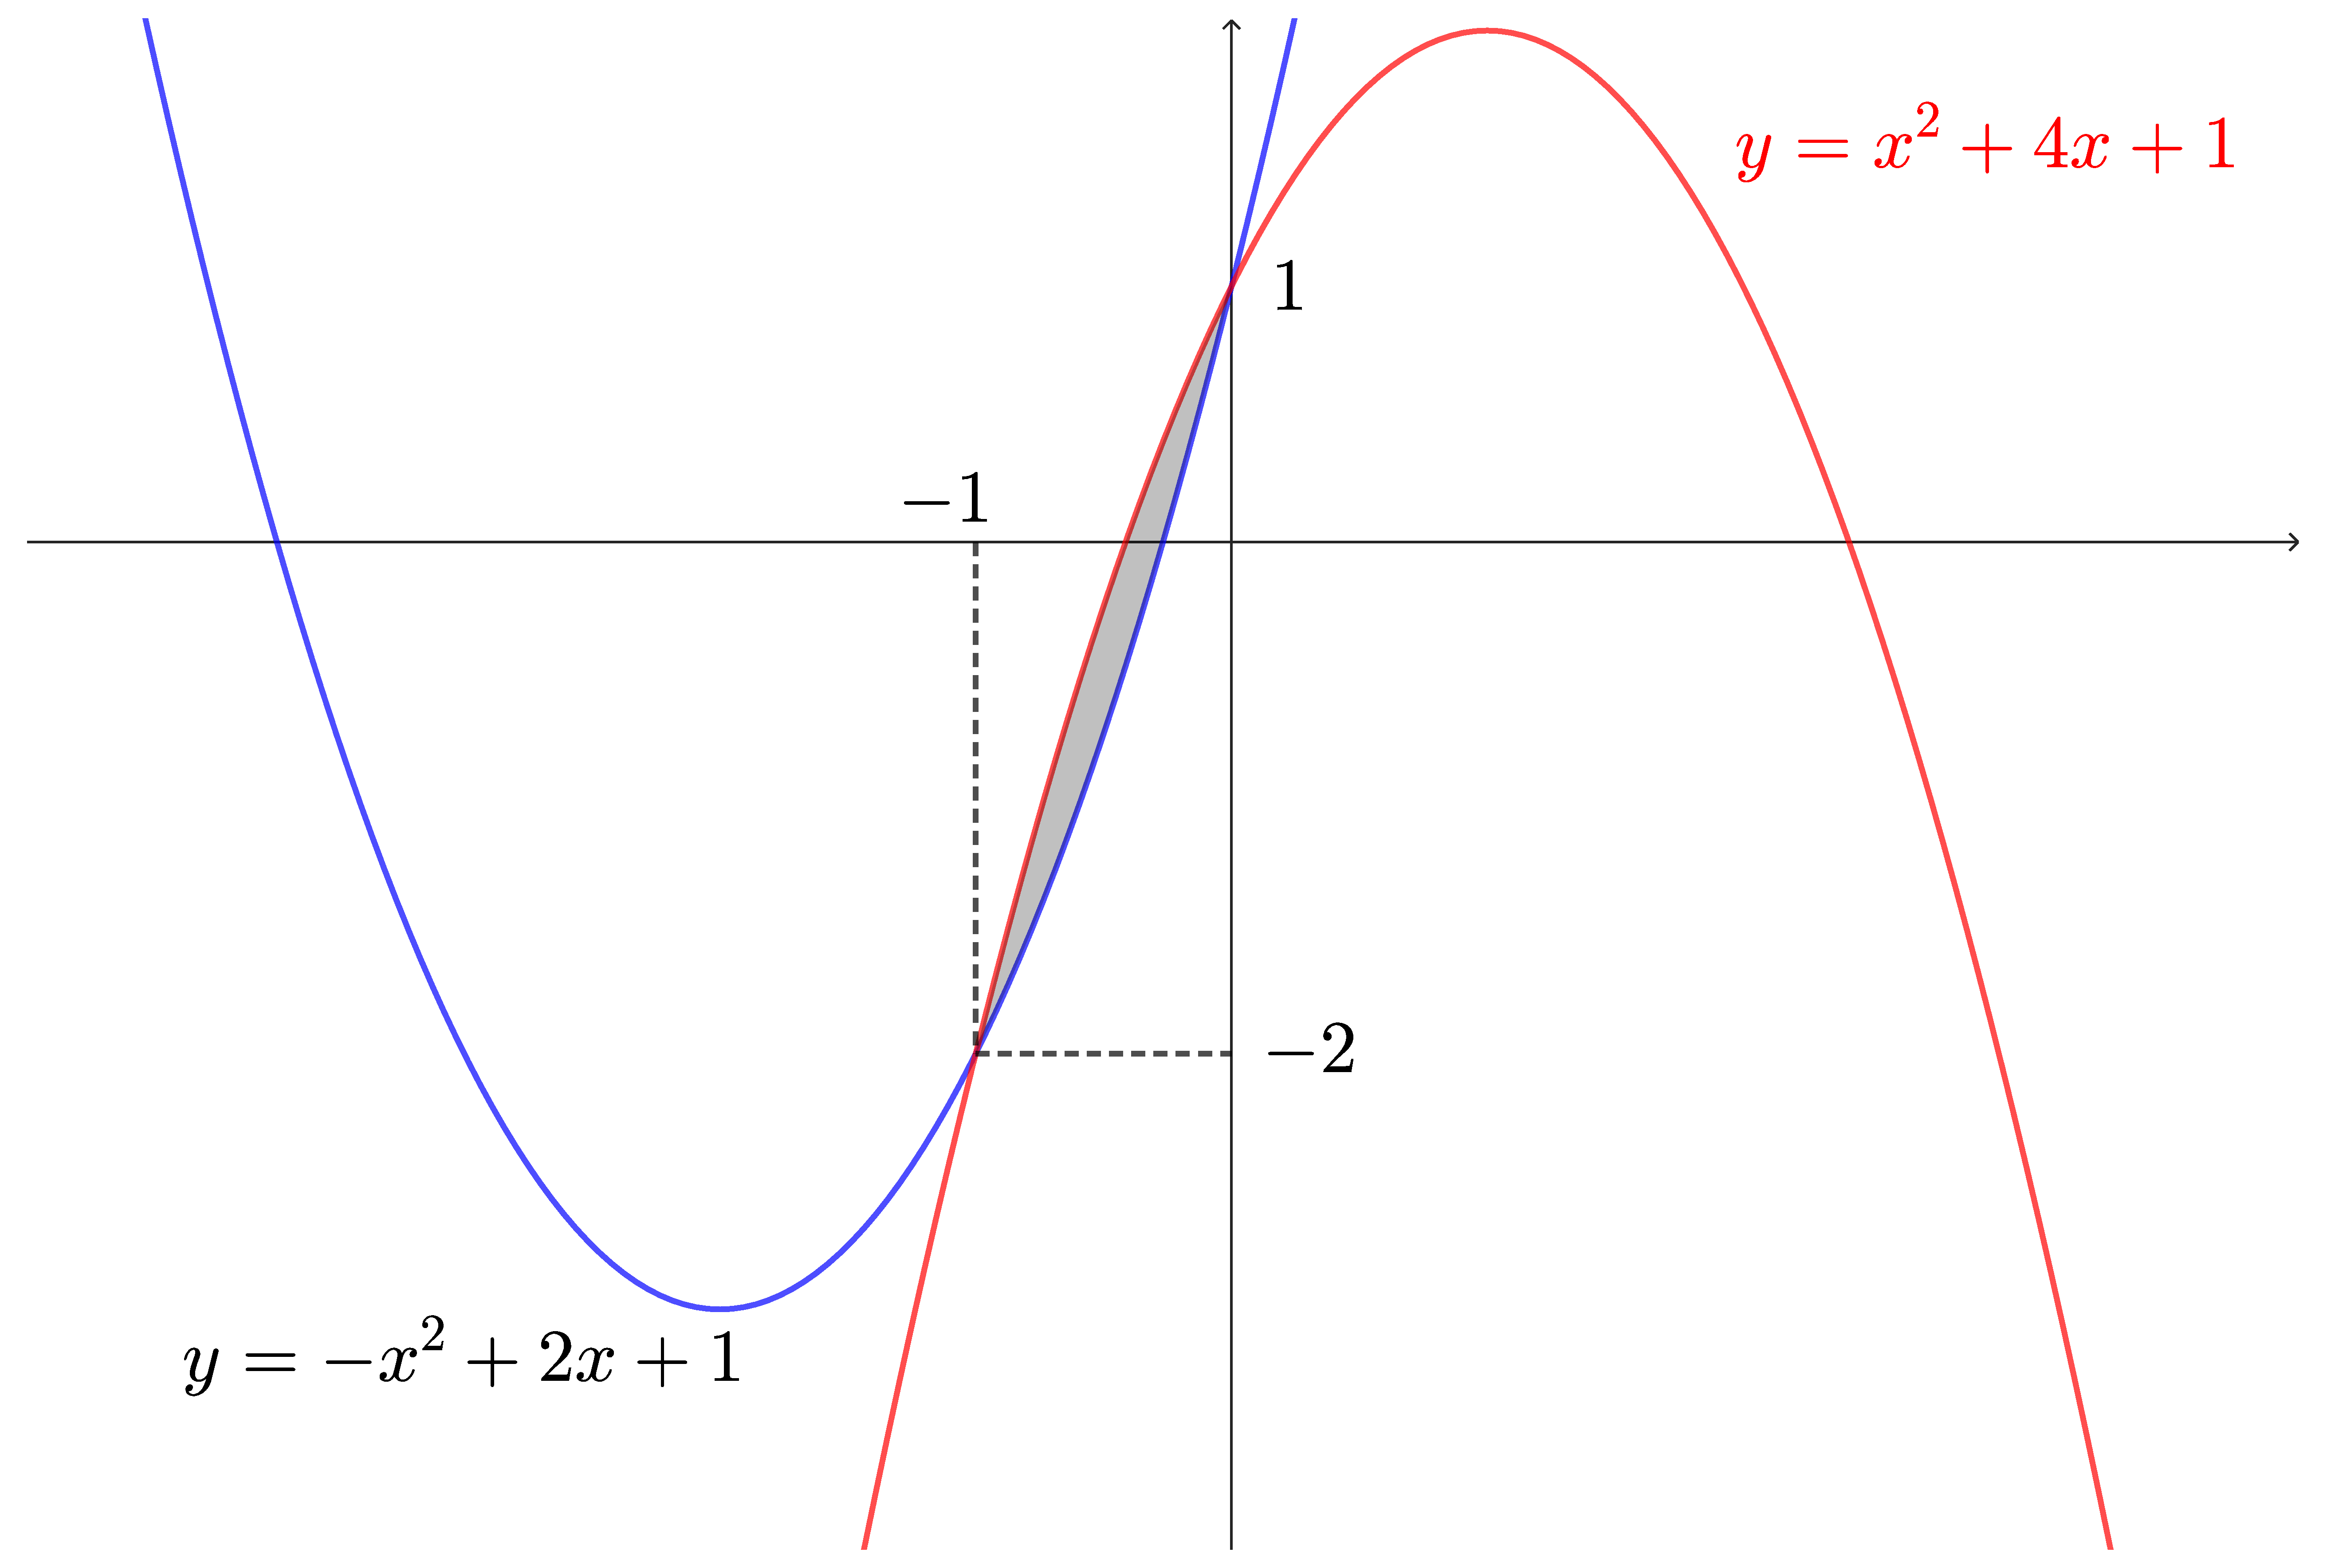
\includegraphics[height=9cm]{./pictures/fig6.pdf}
  \end{figure}

  
  
\end{enumerate}



\end{document}

